\documentclass[aspectratio=169]{beamer}

% -------------------------
% Basic packages
% -------------------------
\usepackage[utf8]{inputenc}
\usepackage{graphicx}
\usepackage{amsmath, amssymb}
\usepackage{booktabs}
\usepackage{array}
\usepackage{tikz}
\usepackage{tcolorbox}
\usepackage{hyperref}
\definecolor{questionbg}{RGB}{235, 244, 255}
\definecolor{questionframe}{RGB}{44, 95, 173}
\definecolor{plainbg}{RGB}{241, 249, 241}
\definecolor{plainframe}{RGB}{44, 122, 70}
\definecolor{notationbg}{RGB}{255, 248, 230}
\definecolor{notationframe}{RGB}{176, 118, 0}

\newtcolorbox{questionbox}{
  colback=questionbg,
  colframe=questionframe,
  boxrule=0.7pt,
  arc=1mm,
  fontupper=\small,
  left=1mm,
  right=1mm,
  top=0.4mm,
  bottom=0.4mm
}

\newtcolorbox{plainbox}{
  colback=plainbg,
  colframe=plainframe,
  boxrule=0.7pt,
  arc=1mm,
  fontupper=\small,
  left=1mm,
  right=1mm,
  top=0.4mm,
  bottom=0.4mm
}

\newtcolorbox{notationbox}{
  colback=notationbg,
  colframe=notationframe,
  boxrule=0.7pt,
  arc=1mm,
  fontupper=\small,
  left=1mm,
  right=1mm,
  top=0.4mm,
  bottom=0.4mm
}

\newcommand{\keyquestion}[1]{%
  \begin{questionbox}
  \textbf{Question:} #1
  \end{questionbox}
}

\newcommand{\plainidea}[1]{%
  \begin{plainbox}
  \textbf{Main idea:} #1
  \end{plainbox}
}

\newcommand{\notationblock}[1]{%
  \begin{notationbox}
  \textbf{Symbols used on this slide}\\
  #1
  \end{notationbox}
}

\newcommand{\exercisebreakcontent}[1]{%
  \begin{center}
  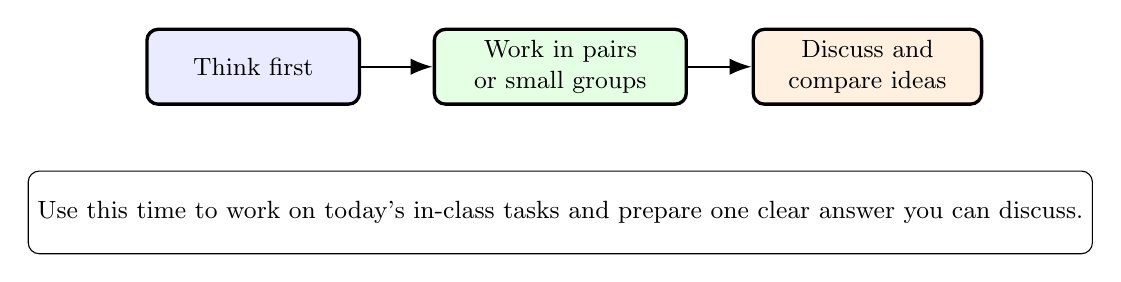
\begin{tikzpicture}[>=Latex, every node/.style={font=\small}]
    \node[draw, rounded corners, very thick, fill=blue!8, minimum width=2.7cm, minimum height=0.95cm, align=center] (think) at (-3.9,0.9) {Think first};
    \node[draw, rounded corners, very thick, fill=green!10, minimum width=3.2cm, minimum height=0.95cm, align=center] (work) at (0,0.9) {Work in pairs\\or small groups};
    \node[draw, rounded corners, very thick, fill=orange!12, minimum width=2.9cm, minimum height=0.95cm, align=center] (share) at (3.9,0.9) {Discuss and\\compare ideas};
    \draw[-{Latex[length=2.8mm]}, thick] (think) -- (work);
    \draw[-{Latex[length=2.8mm]}, thick] (work) -- (share);
    \node[draw, rounded corners, fill=white, minimum width=9.4cm, minimum height=1.05cm, align=center] at (0,-0.95) {Use this time to work on today's in-class tasks and prepare one clear answer you can discuss.};
  \end{tikzpicture}
  \end{center}
  \plainidea{#1}
}

\usetikzlibrary{positioning,arrows.meta,calc,shapes.geometric}

% -------------------------
% Theme
% -------------------------
\usetheme{Madrid}
\usecolortheme{default}
\setbeamertemplate{navigation symbols}{}

% -------------------------
% Per-slide reference footer
% -------------------------
\newcommand{\defaultdeckrefs}{AIMA4e Ch.16--17; Poole3e Ch.12}
\newcommand{\currentsliderefs}{\defaultdeckrefs}
\newcommand{\setslideref}[1]{\gdef\currentsliderefs{#1}}
\addtobeamertemplate{footline}{}{%
  \begin{beamercolorbox}[wd=\paperwidth,leftskip=0.4em,rightskip=0.4em,ht=2.8ex,dp=0.9ex]{author in head/foot}
    \tiny\textbf{Refs: }\currentsliderefs
  \end{beamercolorbox}
}

% -------------------------
% Metadata
% -------------------------
\title[EBU6505 B4 D4]{EBU6505 -- Reasoning and Agents\\Block 4, Day 4 -- Planning with Uncertainty}
\author{Dr Riasat Islam}
\institute{Queen Mary University of London}
\date{}

% -------------------------
% TikZ styles
% -------------------------
\tikzset{
  flowarrow/.style={-{Latex[length=2.8mm]}, thick},
  chance/.style={draw, ellipse, very thick, fill=blue!10, minimum width=2.6cm, minimum height=1.0cm, align=center},
  decision/.style={draw, rounded corners=1mm, very thick, fill=green!12, minimum width=2.7cm, minimum height=1.0cm, align=center},
  utility/.style={draw, diamond, aspect=2.0, very thick, fill=orange!12, minimum width=2.8cm, minimum height=1.0cm, align=center},
  statebox/.style={draw, rounded corners, very thick, fill=blue!10, minimum width=2.3cm, minimum height=0.95cm, align=center},
  actionbox/.style={draw, rounded corners, very thick, fill=green!12, minimum width=2.3cm, minimum height=0.95cm, align=center},
  rewardbox/.style={draw, rounded corners, very thick, fill=orange!12, minimum width=2.3cm, minimum height=0.95cm, align=center},
  beliefbox/.style={draw, rounded corners, very thick, fill=purple!10, minimum width=2.5cm, minimum height=0.95cm, align=center},
  softbox/.style={draw, rounded corners, fill=white, minimum width=2.8cm, minimum height=0.95cm, align=center},
  note/.style={draw, rounded corners, fill=white, minimum width=2.8cm, minimum height=0.85cm, align=center, font=\small}
}

\begin{document}

\setslideref{AIMA4e Ch.16--17; Poole3e Ch.12}
\begin{frame}
  \titlepage
\end{frame}

\begin{frame}{What have we covered this week?}
\begin{itemize}
  \item Day 1: Bayesian networks for static uncertain reasoning
  \item Day 2: exact inference with enumeration and variable elimination
  \item Day 3: temporal models such as hidden Markov models (HMMs), Kalman filters, and dynamic Bayesian networks (DBNs)
\end{itemize}
\plainidea{So far we have focused on belief. Today we move from belief to action.}
\end{frame}

\begin{frame}{What are we going to cover this week?}
\begin{itemize}
  \item Day 1: Bayesian networks
  \item Day 2: exact inference in Bayesian networks
  \item Day 3: probabilistic reasoning over time
  \item Day 4: planning with uncertainty
  \item Day 5: dynamic decision network (DDN) and partially observable Markov decision process (POMDP) synthesis
\end{itemize}
\plainidea{This week moves from uncertain belief, to temporal belief, and then to decision-making.}
\end{frame}

\begin{frame}{What are we going to cover today?}
\begin{itemize}
  \item utility and expected utility
  \item one-off decisions and decision networks
  \item sequential decisions with Markov decision process (MDP) planning
  \item value iteration and policy iteration
  \item why partial observability leads to belief-state planning
\end{itemize}
\plainidea{The lecture has one simple flow: preferences, decisions, planning, then the bridge to partially observable Markov decision processes.}
\end{frame}

\begin{frame}{Resources}
\begin{itemize}
  \item \textit{Artificial Intelligence: A Modern Approach}, 4th ed.\\
  Chapter 16: Making Simple Decisions\\
  Chapter 17: Making Complex Decisions
  \item \textit{Artificial Intelligence: Foundations of Computational Agents}, 3rd ed.\\
  Chapter 12: Planning with Uncertainty
\end{itemize}
\plainidea{These readings match today's flow: one-off decisions first, then sequential decision processes.}
\end{frame}

\begin{frame}{Learning Outcomes for Today}
By the end of this session, you should be able to:
\begin{itemize}
  \item explain utility and expected utility in simple language
  \item distinguish one-off decisions from sequential decisions
  \item explain planning in a Markov decision process (MDP) with a known model
  \item compare value iteration and policy iteration
  \item explain why partial observability leads to belief-state planning
\end{itemize}
\end{frame}

\begin{frame}{Why Plan Under Uncertainty?}
\keyquestion{Why is choosing an action hard when the world is uncertain?}
\begin{columns}[T,onlytextwidth]
  \begin{column}{0.50\textwidth}
    \begin{tcolorbox}[colback=plainbg,colframe=plainframe,boxrule=0.7pt,title=Reality]
    the true world state may be uncertain\\
    actions may have uncertain results
    \end{tcolorbox}
    \begin{tcolorbox}[colback=questionbg,colframe=questionframe,boxrule=0.7pt,title=Consequence]
    a good action now can create better future choices later
    \end{tcolorbox}
  \end{column}
  \begin{column}{0.44\textwidth}
    \begin{center}
    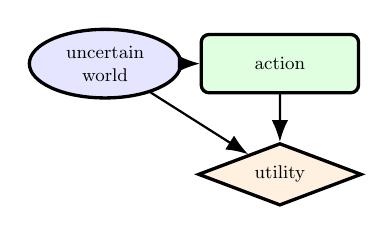
\begin{tikzpicture}[>=Latex, scale=0.74, every node/.style={font=\small, transform shape}]
      \node[chance] (w) at (0,1.0) {uncertain\\world};
      \node[decision] (a) at (3.0,1.0) {action};
      \node[utility] (u) at (3.0,-0.9) {utility};
      \draw[flowarrow] (w) -- (a);
      \draw[flowarrow] (w) -- (u);
      \draw[flowarrow] (a) -- (u);
    \end{tikzpicture}
    \end{center}
  \end{column}
\end{columns}
\vspace{-0.2em}
\plainidea{Planning under uncertainty means choosing actions that are good on average.}
\end{frame}

\begin{frame}{What Is Utility?}
\keyquestion{How do we tell the model which outcomes we prefer?}
\begin{columns}[T,onlytextwidth]
  \begin{column}{0.54\textwidth}
    \begin{tcolorbox}[colback=plainbg,colframe=plainframe,boxrule=0.7pt,title=Simple meaning]
    Utility is a score for how good or bad an outcome is.
    \end{tcolorbox}
    \begin{tcolorbox}[colback=questionbg,colframe=questionframe,boxrule=0.7pt,title=Example]
    A robot may prefer fast delivery, low energy cost, and safe motion.
    \end{tcolorbox}
  \end{column}
  \begin{column}{0.42\textwidth}
    \small
    \begin{center}
    \begin{tabular}{>{\raggedright\arraybackslash}p{0.48\textwidth} c}
    \toprule
    outcome & utility \\
    \midrule
    fast and safe delivery & 10 \\
    safe but slow delivery & 7 \\
    delay or extra cost & 3 \\
    unsafe outcome & -20 \\
    \bottomrule
    \end{tabular}
    \end{center}
  \end{column}
\end{columns}
\plainidea{Utility turns vague preferences into numbers the planner can compare.}
\end{frame}

\begin{frame}{Expected Utility}
\keyquestion{How do we compare actions when each action can lead to more than one outcome?}
\begin{columns}[T,onlytextwidth]
  \begin{column}{0.52\textwidth}
    \[
    EU(a)=\sum_{s'} P(s' \mid a)\,U(s')
    \]
    \notationblock{$EU(a)$: expected utility of action $a$\\
$P(s' \mid a)$: probability of possible outcome $s'$\\
$U(s')$: utility of that outcome}
  \end{column}
  \begin{column}{0.44\textwidth}
    \begin{tcolorbox}[colback=plainbg,colframe=plainframe,boxrule=0.7pt,title=Interpretation]
    Multiply each possible outcome by how likely it is, then add them together.
    \end{tcolorbox}
  \end{column}
\end{columns}
\plainidea{Expected utility is the average score of an action after uncertainty is taken into account.}
\end{frame}

\begin{frame}{A Small Expected-Utility Example}
\keyquestion{Which route should the delivery robot choose?}
\small
\begin{center}
\begin{tabular}{>{\raggedright\arraybackslash}p{0.18\textwidth} >{\raggedright\arraybackslash}p{0.28\textwidth} >{\raggedright\arraybackslash}p{0.18\textwidth} >{\raggedright\arraybackslash}p{0.16\textwidth}}
\toprule
action & possible outcome & probability & utility \\
\midrule
fast route & clear road & 0.6 & 10 \\
fast route & traffic delay & 0.4 & 2 \\
safe route & normal arrival & 1.0 & 7 \\
\bottomrule
\end{tabular}
\end{center}
\begin{columns}[T,onlytextwidth]
  \begin{column}{0.48\textwidth}
    \begin{tcolorbox}[colback=questionbg,colframe=questionframe,boxrule=0.7pt,title=Fast route]
    $EU = 0.6(10)+0.4(2)=6.8$
    \end{tcolorbox}
  \end{column}
  \begin{column}{0.48\textwidth}
    \begin{tcolorbox}[colback=plainbg,colframe=plainframe,boxrule=0.7pt,title=Safe route]
    $EU = 1.0(7)=7$
    \end{tcolorbox}
  \end{column}
\end{columns}
\plainidea{The safe route wins because its average utility is slightly higher.}
\end{frame}

\begin{frame}{What Is the Value of Information?}
\keyquestion{When is it worth spending time or cost to learn more before acting?}
\begin{columns}[T,onlytextwidth]
  \begin{column}{0.48\textwidth}
    \begin{tcolorbox}[colback=plainbg,colframe=plainframe,boxrule=0.7pt,title=Without extra information]
    choose one action now using current uncertainty
    \end{tcolorbox}
    \begin{tcolorbox}[colback=questionbg,colframe=questionframe,boxrule=0.7pt,title=With extra information]
    observe first, reduce uncertainty, then choose an action
    \end{tcolorbox}
  \end{column}
  \begin{column}{0.48\textwidth}
    \begin{center}
    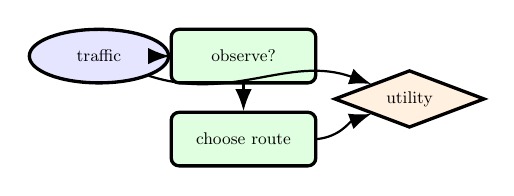
\begin{tikzpicture}[>=Latex, scale=0.68, every node/.style={font=\small, transform shape}]
      \node[chance] (traffic) at (0,1.2) {traffic};
      \node[decision] (observe) at (2.7,1.2) {observe?};
      \node[decision] (route) at (2.7,-0.35) {choose route};
      \node[utility] (u) at (5.8,0.4) {utility};
      \draw[flowarrow] (traffic.east) -- (observe.west);
      \draw[flowarrow] (observe.south) -- (route.north);
      \draw[flowarrow] (traffic.south east) to[out=-18,in=160] (u.north west);
      \draw[flowarrow] (route.east) to[out=6,in=-160] (u.south west);
    \end{tikzpicture}
    \end{center}
  \end{column}
\end{columns}
\plainidea{Information has value when better knowledge can change the action and improve utility.}
\end{frame}

\begin{frame}{Decision Trees}
\keyquestion{How can we write down a simple one-off decision problem step by step?}
\begin{center}
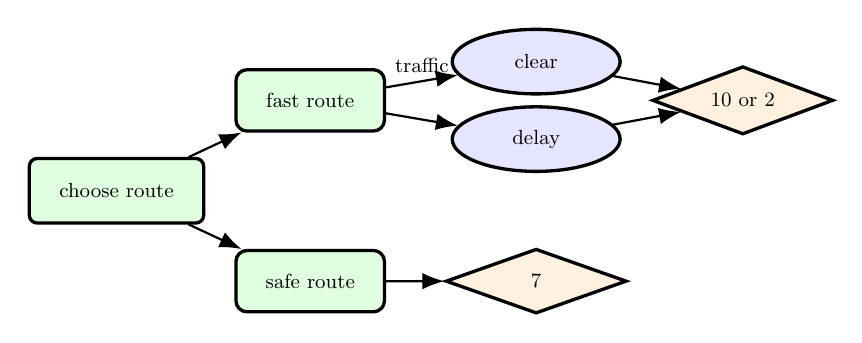
\begin{tikzpicture}[>=Latex, scale=0.82, every node/.style={font=\small, transform shape}]
  \node[decision] (start) at (0,0) {choose route};
  \node[actionbox] (fast) at (3.0,1.4) {fast route};
  \node[actionbox] (safe) at (3.0,-1.4) {safe route};
  \node[chance] (clear) at (6.5,2.0) {clear};
  \node[chance] (delay) at (6.5,0.8) {delay};
  \node[utility] (uf) at (9.7,1.4) {10 or 2};
  \node[utility] (us) at (6.5,-1.4) {7};
  \draw[flowarrow] (start) -- (fast);
  \draw[flowarrow] (start) -- (safe);
  \draw[flowarrow] (fast) -- node[above, font=\small] {traffic} (clear);
  \draw[flowarrow] (fast) -- (delay);
  \draw[flowarrow] (clear) -- (uf);
  \draw[flowarrow] (delay) -- (uf);
  \draw[flowarrow] (safe) -- (us);
\end{tikzpicture}
\end{center}
\plainidea{A decision tree makes the order of decision, uncertainty, and utility explicit.}
\end{frame}

\begin{frame}{Decision Networks}
\keyquestion{How do we show the same problem more compactly?}
\begin{columns}[T,onlytextwidth]
  \begin{column}{0.50\textwidth}
    \begin{tcolorbox}[colback=plainbg,colframe=plainframe,boxrule=0.7pt,title=Node meanings]
    \small
    \textbf{Chance node}: uncertain part of the world\\[0.2em]
    \textbf{Decision node}: choice the agent can make\\[0.2em]
    \textbf{Utility node}: final score of the result
    \end{tcolorbox}
  \end{column}
  \begin{column}{0.44\textwidth}
    \begin{center}
    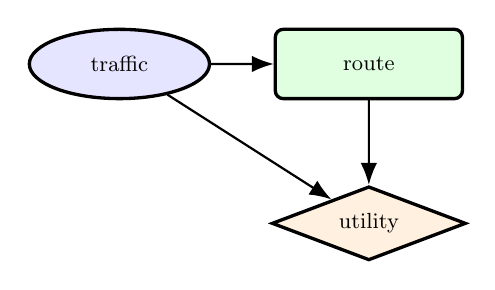
\begin{tikzpicture}[>=Latex, scale=0.88, every node/.style={font=\small, transform shape}]
      \node[chance] (w) at (0,1.3) {traffic};
      \node[decision] (d) at (3.6,1.3) {route};
      \node[utility] (u) at (3.6,-1.0) {utility};
      \draw[flowarrow] (w) -- (d);
      \draw[flowarrow] (w) -- (u);
      \draw[flowarrow] (d) -- (u);
    \end{tikzpicture}
    \end{center}
  \end{column}
\end{columns}
\plainidea{A decision network shows the same logic as a tree in a compact graph.}
\end{frame}

\begin{frame}{One-Off Decisions vs Sequential Decisions}
\keyquestion{What changes when the agent acts more than once?}
\begin{columns}[T,onlytextwidth]
  \begin{column}{0.48\textwidth}
    \begin{tcolorbox}[colback=plainbg,colframe=plainframe,boxrule=0.7pt,title=One-off decision]
    one action\\
    one uncertainty calculation\\
    choose once
    \end{tcolorbox}
  \end{column}
  \begin{column}{0.48\textwidth}
    \begin{tcolorbox}[colback=questionbg,colframe=questionframe,boxrule=0.7pt,title=Sequential decision]
    many actions over time\\
    current action changes future state\\
    need a policy
    \end{tcolorbox}
  \end{column}
\end{columns}
\plainidea{Sequential planning is harder because the agent must care about future consequences, not only the next step.}
\end{frame}

\begin{frame}{MDP Components Refresher}
\keyquestion{Which five pieces define a planning problem as a Markov decision process (MDP)?}
\[
\mathcal{M}=(S,A,T,R,\gamma)
\]
\begin{center}
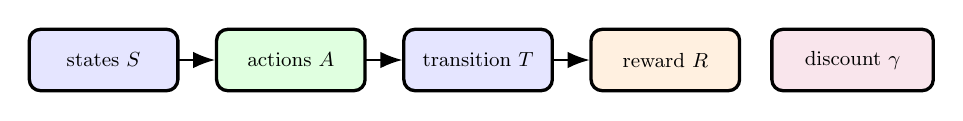
\begin{tikzpicture}[>=Latex, scale=0.82, every node/.style={font=\small, transform shape}]
  \node[statebox] (s) at (0,0) {states $S$};
  \node[actionbox] (a) at (2.9,0) {actions $A$};
  \node[statebox] (t) at (5.8,0) {transition $T$};
  \node[rewardbox] (r) at (8.7,0) {reward $R$};
  \node[beliefbox] (g) at (11.6,0) {discount $\gamma$};
  \draw[flowarrow] (s) -- (a);
  \draw[flowarrow] (a) -- (t);
  \draw[flowarrow] (t) -- (r);
\end{tikzpicture}
\end{center}
\notationblock{$S$: possible states\\
$A$: possible actions\\
$T(s,a,s')$: probability of next state\\
$R(s,a,s')$: immediate reward\\
$\gamma$: how much future reward matters}
\plainidea{A Markov decision process (MDP) is the standard model for sequential planning when the state is fully observable.}
\end{frame}

\begin{frame}{Planning in an MDP Is Not RL}
\keyquestion{What is the difference between planning in a Markov decision process and learning in one?}
\begin{columns}[T,onlytextwidth]
  \begin{column}{0.48\textwidth}
    \begin{tcolorbox}[colback=plainbg,colframe=plainframe,boxrule=0.7pt,title=Planning]
    the model is known\\
    compute good values and policies from the model
    \end{tcolorbox}
  \end{column}
  \begin{column}{0.48\textwidth}
    \begin{tcolorbox}[colback=questionbg,colframe=questionframe,boxrule=0.7pt,title=Reinforcement learning]
    the model is unknown\\
    learn from experience and feedback
    \end{tcolorbox}
  \end{column}
\end{columns}
\plainidea{Today we are not learning the model. We are planning with a model that is already given.}
\end{frame}

\begin{frame}{What Is the Planner Maximising?}
\keyquestion{What is the long-term quantity the planner wants to make as large as possible?}
\[
G_t=\sum_{k=0}^{\infty}\gamma^k r_{t+k+1}
\]
\begin{columns}[T,onlytextwidth]
  \begin{column}{0.52\textwidth}
    \notationblock{$G_t$: total reward from time $t$ onward\\
$r_{t+k+1}$: later reward\\
$\gamma$: weight on future reward}
  \end{column}
  \begin{column}{0.44\textwidth}
    \begin{tcolorbox}[colback=plainbg,colframe=plainframe,boxrule=0.7pt,title=Interpretation]
    high $\gamma$: future reward matters more\\
    low $\gamma$: the planner is more short-term
    \end{tcolorbox}
  \end{column}
\end{columns}
\vspace{-0.35em}
\plainidea{The planner aims to maximise expected long-term return, not just the next reward.}
\end{frame}

\begin{frame}{Bellman Backup Intuition}
\keyquestion{How does the planner compare one action against another in one state?}
\[
V^*(s)=\max_a \sum_{s'} T(s,a,s')\left[R(s,a,s')+\gamma V^*(s')\right]
\]
\begin{center}
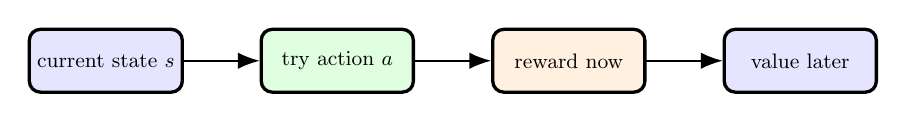
\begin{tikzpicture}[>=Latex, scale=0.84, every node/.style={font=\small, transform shape}]
  \node[statebox] (s) at (0,0) {current state $s$};
  \node[actionbox] (a) at (3.5,0) {try action $a$};
  \node[rewardbox] (r) at (7.0,0) {reward now};
  \node[statebox] (n) at (10.5,0) {value later};
  \draw[flowarrow] (s) -- (a);
  \draw[flowarrow] (a) -- (r);
  \draw[flowarrow] (r) -- (n);
\end{tikzpicture}
\end{center}
\notationblock{$V^*(s)$: best long-term value of state $s$\\
$T(s,a,s')$: chance of each next state\\
$R(s,a,s')$: immediate reward for that transition}
\plainidea{Bellman backup asks: which action gives the best mix of reward now and value later?}
\end{frame}

\begin{frame}{Value Iteration}
\keyquestion{How does value iteration solve the planning problem?}
\begin{center}
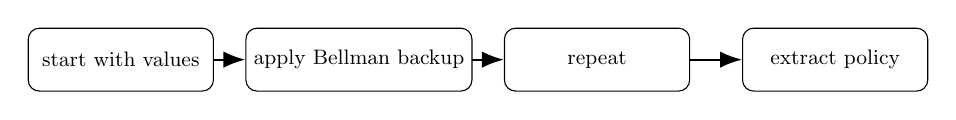
\begin{tikzpicture}[>=Latex, scale=0.84, every node/.style={font=\small, transform shape}]
  \node[softbox] (v0) at (0,0) {start with values};
  \node[softbox] (b) at (3.6,0) {apply Bellman backup};
  \node[softbox] (r) at (7.2,0) {repeat};
  \node[softbox] (p) at (10.8,0) {extract policy};
  \draw[flowarrow] (v0) -- (b);
  \draw[flowarrow] (b) -- (r);
  \draw[flowarrow] (r) -- (p);
\end{tikzpicture}
\end{center}
\begin{columns}[T,onlytextwidth]
  \begin{column}{0.48\textwidth}
    \begin{tcolorbox}[colback=plainbg,colframe=plainframe,boxrule=0.7pt,title=What changes?]
    values for each state
    \end{tcolorbox}
  \end{column}
  \begin{column}{0.48\textwidth}
    \begin{tcolorbox}[colback=questionbg,colframe=questionframe,boxrule=0.7pt,title=When do we stop?]
    when the values change only a little
    \end{tcolorbox}
  \end{column}
\end{columns}
\plainidea{Value iteration improves state values first, then reads the best action from those values.}
\end{frame}

\begin{frame}{A Tiny Value-Iteration Picture}
\keyquestion{What does repeated improvement look like in a very small state space?}
\begin{center}
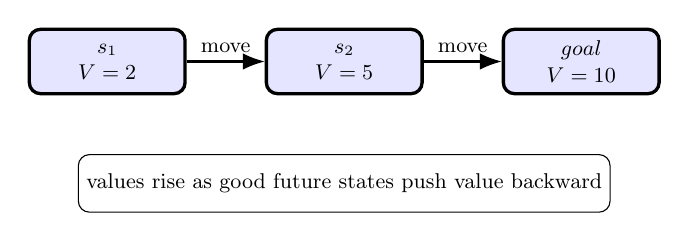
\begin{tikzpicture}[>=Latex, scale=0.86, every node/.style={font=\small, transform shape}]
  \node[statebox] (s1) at (0,0) {$s_1$\\$V=2$};
  \node[statebox] (s2) at (3.5,0) {$s_2$\\$V=5$};
  \node[statebox] (s3) at (7.0,0) {$goal$\\$V=10$};
  \draw[flowarrow] (s1) -- node[above] {move} (s2);
  \draw[flowarrow] (s2) -- node[above] {move} (s3);
  \node[note] at (3.5,-1.8) {values rise as good future states push value backward};
\end{tikzpicture}
\end{center}
\plainidea{Good future states send value backward to earlier states through repeated backups.}
\end{frame}

\begin{frame}{Policy Iteration}
\keyquestion{How does policy iteration differ from value iteration?}
\begin{center}
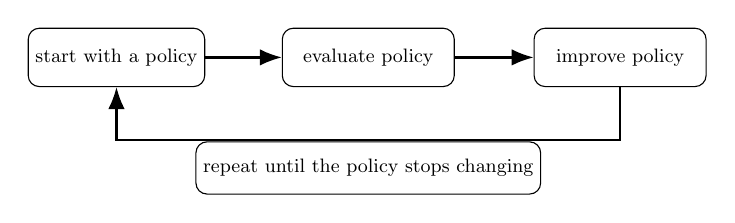
\begin{tikzpicture}[>=Latex, scale=0.78, every node/.style={font=\small, transform shape}]
  \node[softbox] (p0) at (0,0) {start with a policy};
  \node[softbox] (eval) at (4.1,0) {evaluate policy};
  \node[softbox] (imp) at (8.2,0) {improve policy};
  \draw[flowarrow] (p0) -- (eval);
  \draw[flowarrow] (eval) -- (imp);
  \coordinate (loopback) at (4.1,-1.35);
  \draw[flowarrow] (imp.south) |- (loopback) -| (p0.south);
  \node[note] at (4.1,-1.8) {repeat until the policy stops changing};
\end{tikzpicture}
\end{center}
\begin{tcolorbox}[colback=plainbg,colframe=plainframe,boxrule=0.7pt,title=Simple language]
First ask, "How good is this current policy?" Then ask, "Can I improve any action?"
\end{tcolorbox}
\plainidea{Policy iteration alternates between judging one policy and improving it.}
\end{frame}

\begin{frame}{Value Iteration vs Policy Iteration}
\keyquestion{How can we compare the two planning algorithms quickly?}
\small
\begin{center}
\begin{tabular}{>{\raggedright\arraybackslash}p{0.22\textwidth} >{\raggedright\arraybackslash}p{0.30\textwidth} >{\raggedright\arraybackslash}p{0.30\textwidth}}
\toprule
feature & value iteration & policy iteration \\
\midrule
main update & update values directly & evaluate then improve a policy \\
starting point & any initial values & any initial policy \\
common intuition & push values backward & polish a policy step by step \\
\bottomrule
\end{tabular}
\end{center}
\plainidea{Both algorithms solve the same planning problem, but they organise the work differently.}
\end{frame}

\begin{frame}{What Assumption Does an MDP Make?}
\keyquestion{What does the planner assume it knows at decision time?}
\begin{columns}[T,onlytextwidth]
  \begin{column}{0.48\textwidth}
    \begin{tcolorbox}[colback=plainbg,colframe=plainframe,boxrule=0.7pt,title=MDP assumption]
    the agent knows the true current state
    \end{tcolorbox}
  \end{column}
  \begin{column}{0.48\textwidth}
    \begin{tcolorbox}[colback=questionbg,colframe=questionframe,boxrule=0.7pt,title=Problem]
    in real systems the observation may be noisy, delayed, or incomplete
    \end{tcolorbox}
  \end{column}
\end{columns}
\plainidea{MDP planning works well only when the current state is fully observable.}
\end{frame}

\begin{frame}{When Full Observability Breaks}
\keyquestion{What does the agent use if it cannot see the true state directly?}
\begin{center}
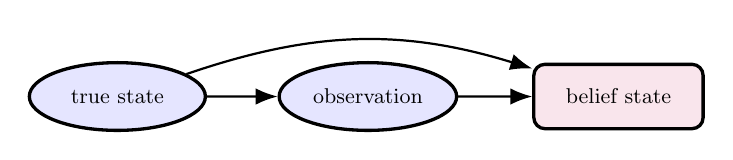
\begin{tikzpicture}[>=Latex, scale=0.86, every node/.style={font=\small, transform shape}]
  \node[chance] (true) at (0,1.0) {true state};
  \node[chance] (obs) at (3.7,1.0) {observation};
  \node[beliefbox] (belief) at (7.4,1.0) {belief state};
  \draw[flowarrow] (true) -- (obs);
  \draw[flowarrow] (obs) -- (belief);
  \draw[flowarrow] (true) to[bend left=18] (belief);
\end{tikzpicture}
\end{center}
\begin{tcolorbox}[colback=plainbg,colframe=plainframe,boxrule=0.7pt,title=Simple meaning]
The agent stores a probability distribution over states instead of one certain state label.
\end{tcolorbox}
\plainidea{Under partial observability, the planner acts on beliefs about state, not on state itself.}
\end{frame}

\begin{frame}{Belief-State Planning Loop}
\keyquestion{How does the agent keep planning when it only has a belief?}
\begin{center}
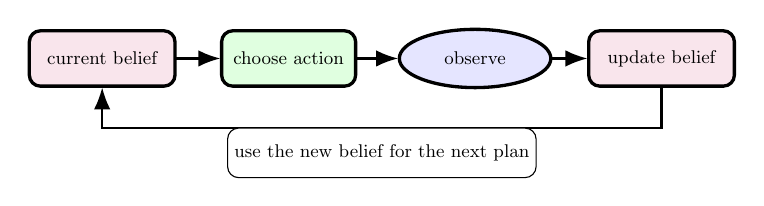
\begin{tikzpicture}[>=Latex, scale=0.74, every node/.style={font=\small, transform shape}]
  \node[beliefbox] (b) at (0,0) {current belief};
  \node[actionbox] (a) at (3.2,0) {choose action};
  \node[chance] (o) at (6.4,0) {observe};
  \node[beliefbox] (u) at (9.6,0) {update belief};
  \draw[flowarrow] (b) -- (a);
  \draw[flowarrow] (a) -- (o);
  \draw[flowarrow] (o) -- (u);
  \coordinate (nextloop) at (4.8,-1.2);
  \draw[flowarrow] (u.south) |- (nextloop) -| (b.south);
  \node[note] at (4.8,-1.62) {use the new belief for the next plan};
\end{tikzpicture}
\end{center}
\plainidea{The loop is: plan, act, observe, update belief, then plan again.}
\end{frame}

\begin{frame}{POMDP Preview}
\keyquestion{What does a partially observable Markov decision process (POMDP) add on top of an MDP?}
\begin{columns}[T,onlytextwidth]
  \begin{column}{0.48\textwidth}
    \begin{tcolorbox}[colback=plainbg,colframe=plainframe,boxrule=0.7pt,title=MDP]
    states, actions, transitions, rewards, discount
    \end{tcolorbox}
  \end{column}
  \begin{column}{0.48\textwidth}
    \begin{tcolorbox}[colback=questionbg,colframe=questionframe,boxrule=0.7pt,title=POMDP]
    all of the above, plus hidden state and an observation model
    \end{tcolorbox}
  \end{column}
\end{columns}
\notationblock{$b_t(s)=P(s_t=s \mid o_{1:t},a_{1:t-1})$: belief that state $s$ is true at time $t$}
\plainidea{A partially observable Markov decision process (POMDP) is a planning model for acting under uncertainty when the true state is not directly visible.}
\end{frame}

\begin{frame}{Which Model Fits Which Situation?}
\keyquestion{How do we know whether we need a decision network, an MDP, or a POMDP?}
\small
\begin{center}
\begin{tabular}{>{\raggedright\arraybackslash}p{0.22\textwidth} >{\raggedright\arraybackslash}p{0.22\textwidth} >{\raggedright\arraybackslash}p{0.38\textwidth}}
\toprule
model & best for & simple description \\
\midrule
decision network & one-off decision & choose once under uncertainty \\
MDP & sequential, fully observed & choose many times with known current state \\
POMDP & sequential, partially observed & choose many times using belief instead of true state \\
\bottomrule
\end{tabular}
\end{center}
\plainidea{The right model depends on whether decisions are one-off or sequential, and whether the state is visible or hidden.}
\end{frame}

\begin{frame}{A Simple Running Scenario}
\keyquestion{How do all these models appear in one delivery-robot story?}
\begin{columns}[T,onlytextwidth]
  \begin{column}{0.54\textwidth}
    \begin{tcolorbox}[colback=plainbg,colframe=plainframe,boxrule=0.7pt,title=Three views of the same story]
    \small
    \textbf{Decision network}: choose a route once under uncertain traffic\\[0.2em]
    \textbf{MDP}: choose move, wait, or recharge over many steps\\[0.2em]
    \textbf{POMDP}: plan with belief when battery or traffic is only partly visible
    \end{tcolorbox}
  \end{column}
  \begin{column}{0.40\textwidth}
    \begin{center}
    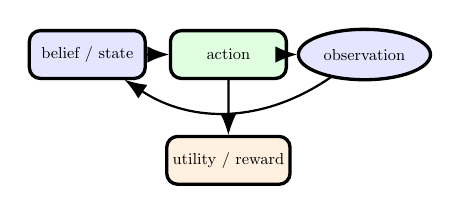
\begin{tikzpicture}[>=Latex, scale=0.64, every node/.style={font=\small, transform shape}]
      \node[statebox] (s) at (0,1.4) {belief / state};
      \node[actionbox] (a) at (2.8,1.4) {action};
      \node[chance] (o) at (5.5,1.4) {observation};
      \node[rewardbox] (r) at (2.8,-0.7) {utility / reward};
      \draw[flowarrow] (s) -- (a);
      \draw[flowarrow] (a) -- (o);
      \draw[flowarrow] (a) -- (r);
      \draw[flowarrow] (o) to[bend left=34] (s);
    \end{tikzpicture}
    \end{center}
  \end{column}
\end{columns}
\vspace{-0.25em}
\plainidea{These are different views of the same uncertain decision problem.}
\end{frame}

\begin{frame}{What Can Go Wrong?}
\keyquestion{Why can planning under uncertainty still fail?}
\begin{columns}[T,onlytextwidth]
  \begin{column}{0.48\textwidth}
    \begin{tcolorbox}[colback=questionbg,colframe=questionframe,boxrule=0.7pt,title=Common problems]
    wrong model\\
    wrong utilities\\
    missing observations\\
    overconfidence in noisy evidence
    \end{tcolorbox}
  \end{column}
  \begin{column}{0.48\textwidth}
    \begin{tcolorbox}[colback=plainbg,colframe=plainframe,boxrule=0.7pt,title=Why it matters]
    the planner may choose an action that looks optimal in the model but is poor in the real world
    \end{tcolorbox}
  \end{column}
\end{columns}
\plainidea{A mathematically correct planner can still make bad decisions if the model or utility is wrong.}
\end{frame}

\begin{frame}{Simple Safety Checks}
\keyquestion{How do we make uncertain planning safer in real systems?}
\begin{columns}[T,onlytextwidth]
  \begin{column}{0.48\textwidth}
    \begin{tcolorbox}[colback=plainbg,colframe=plainframe,boxrule=0.7pt,title=Model-side checks]
    calibrate probabilities\\
    monitor model drift\\
    test utility assumptions
    \end{tcolorbox}
  \end{column}
  \begin{column}{0.48\textwidth}
    \begin{tcolorbox}[colback=questionbg,colframe=questionframe,boxrule=0.7pt,title=Decision-side checks]
    keep a safe fallback action\\
    ask for more evidence when risk is high\\
    use human approval for costly actions
    \end{tcolorbox}
  \end{column}
\end{columns}
\plainidea{Good planning under uncertainty needs both a good model and sensible safety controls.}
\end{frame}

\begin{frame}{Where Are We Going Next?}
\keyquestion{What changes when the uncertainty is both temporal and partially observed?}
\begin{columns}[T,onlytextwidth]
  \begin{column}{0.52\textwidth}
    \begin{tcolorbox}[colback=plainbg,colframe=plainframe,boxrule=0.7pt,title=Today]
    probabilities, utilities, decision networks, and MDP planning
    \end{tcolorbox}
    \begin{tcolorbox}[colback=questionbg,colframe=questionframe,boxrule=0.7pt,title=Next lecture]
    integrate temporal belief, decision nodes, and POMDP ideas into one synthesis
    \end{tcolorbox}
  \end{column}
  \begin{column}{0.42\textwidth}
    \begin{center}
    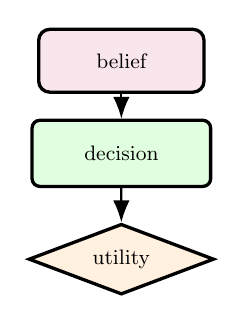
\begin{tikzpicture}[>=Latex, scale=0.84, every node/.style={font=\small, transform shape}]
      \node[beliefbox] (b) at (0,1.3) {belief};
      \node[decision] (d) at (0,-0.1) {decision};
      \node[utility] (u) at (0,-1.7) {utility};
      \draw[flowarrow] (b) -- (d);
      \draw[flowarrow] (d) -- (u);
    \end{tikzpicture}
    \end{center}
  \end{column}
\end{columns}
\plainidea{Day 5 combines belief over time with decision-making under uncertainty.}
\end{frame}

\begin{frame}{In-Class Exercises}
\exercisebreakcontent{Use the exercise time to decide which planning model fits each scenario and explain your choice clearly.}
\end{frame}

\begin{frame}{Summary}
\begin{itemize}
  \item utility and expected utility support one-off decision-making under uncertainty
  \item decision networks give a compact graphical view of decisions plus uncertainty
  \item MDPs support sequential planning when the current state is known
  \item value iteration and policy iteration are two standard planning algorithms
  \item POMDPs are needed when the true state is hidden and the agent must plan with belief
\end{itemize}
\plainidea{Planning with uncertainty means connecting probability, preference, and future consequences in one decision model.}
\end{frame}

\begin{frame}{Further Study}
\begin{itemize}
  \item Read Poole Chapter 12 and AIMA Chapters 16--17.
  \item Practice: Poole Ch.12, Exercises 12.2, 12.3, 12.6, 12.8, 12.13, and 12.15.
  \item AIMA decision-theory exercise page: 16.19, 16.20, 16.21, and 16.22.
  \item AIMA complex-decisions exercise page: 17.1, 17.8, and 17.14.
  \item Focus on expected utility, decision-network structure, and the difference between one-off choice and Markov decision process planning.
\end{itemize}
\end{frame}

\end{document}
